\documentclass[]{book}
\usepackage{lmodern}
\usepackage{amssymb,amsmath}
\usepackage{ifxetex,ifluatex}
\usepackage{fixltx2e} % provides \textsubscript
\ifnum 0\ifxetex 1\fi\ifluatex 1\fi=0 % if pdftex
  \usepackage[T1]{fontenc}
  \usepackage[utf8]{inputenc}
\else % if luatex or xelatex
  \ifxetex
    \usepackage{mathspec}
  \else
    \usepackage{fontspec}
  \fi
  \defaultfontfeatures{Ligatures=TeX,Scale=MatchLowercase}
\fi
% use upquote if available, for straight quotes in verbatim environments
\IfFileExists{upquote.sty}{\usepackage{upquote}}{}
% use microtype if available
\IfFileExists{microtype.sty}{%
\usepackage{microtype}
\UseMicrotypeSet[protrusion]{basicmath} % disable protrusion for tt fonts
}{}
\usepackage[margin=1in]{geometry}
\usepackage{hyperref}
\hypersetup{unicode=true,
            pdftitle={A Reproducible Research Compendium},
            pdfauthor={cf.~list of contributors at https://github.com/rr-mrc-bsu/reproducible-research/graphs/contributors},
            pdfborder={0 0 0},
            breaklinks=true}
\urlstyle{same}  % don't use monospace font for urls
\usepackage{natbib}
\bibliographystyle{apalike}
\usepackage{color}
\usepackage{fancyvrb}
\newcommand{\VerbBar}{|}
\newcommand{\VERB}{\Verb[commandchars=\\\{\}]}
\DefineVerbatimEnvironment{Highlighting}{Verbatim}{commandchars=\\\{\}}
% Add ',fontsize=\small' for more characters per line
\usepackage{framed}
\definecolor{shadecolor}{RGB}{248,248,248}
\newenvironment{Shaded}{\begin{snugshade}}{\end{snugshade}}
\newcommand{\KeywordTok}[1]{\textcolor[rgb]{0.13,0.29,0.53}{\textbf{#1}}}
\newcommand{\DataTypeTok}[1]{\textcolor[rgb]{0.13,0.29,0.53}{#1}}
\newcommand{\DecValTok}[1]{\textcolor[rgb]{0.00,0.00,0.81}{#1}}
\newcommand{\BaseNTok}[1]{\textcolor[rgb]{0.00,0.00,0.81}{#1}}
\newcommand{\FloatTok}[1]{\textcolor[rgb]{0.00,0.00,0.81}{#1}}
\newcommand{\ConstantTok}[1]{\textcolor[rgb]{0.00,0.00,0.00}{#1}}
\newcommand{\CharTok}[1]{\textcolor[rgb]{0.31,0.60,0.02}{#1}}
\newcommand{\SpecialCharTok}[1]{\textcolor[rgb]{0.00,0.00,0.00}{#1}}
\newcommand{\StringTok}[1]{\textcolor[rgb]{0.31,0.60,0.02}{#1}}
\newcommand{\VerbatimStringTok}[1]{\textcolor[rgb]{0.31,0.60,0.02}{#1}}
\newcommand{\SpecialStringTok}[1]{\textcolor[rgb]{0.31,0.60,0.02}{#1}}
\newcommand{\ImportTok}[1]{#1}
\newcommand{\CommentTok}[1]{\textcolor[rgb]{0.56,0.35,0.01}{\textit{#1}}}
\newcommand{\DocumentationTok}[1]{\textcolor[rgb]{0.56,0.35,0.01}{\textbf{\textit{#1}}}}
\newcommand{\AnnotationTok}[1]{\textcolor[rgb]{0.56,0.35,0.01}{\textbf{\textit{#1}}}}
\newcommand{\CommentVarTok}[1]{\textcolor[rgb]{0.56,0.35,0.01}{\textbf{\textit{#1}}}}
\newcommand{\OtherTok}[1]{\textcolor[rgb]{0.56,0.35,0.01}{#1}}
\newcommand{\FunctionTok}[1]{\textcolor[rgb]{0.00,0.00,0.00}{#1}}
\newcommand{\VariableTok}[1]{\textcolor[rgb]{0.00,0.00,0.00}{#1}}
\newcommand{\ControlFlowTok}[1]{\textcolor[rgb]{0.13,0.29,0.53}{\textbf{#1}}}
\newcommand{\OperatorTok}[1]{\textcolor[rgb]{0.81,0.36,0.00}{\textbf{#1}}}
\newcommand{\BuiltInTok}[1]{#1}
\newcommand{\ExtensionTok}[1]{#1}
\newcommand{\PreprocessorTok}[1]{\textcolor[rgb]{0.56,0.35,0.01}{\textit{#1}}}
\newcommand{\AttributeTok}[1]{\textcolor[rgb]{0.77,0.63,0.00}{#1}}
\newcommand{\RegionMarkerTok}[1]{#1}
\newcommand{\InformationTok}[1]{\textcolor[rgb]{0.56,0.35,0.01}{\textbf{\textit{#1}}}}
\newcommand{\WarningTok}[1]{\textcolor[rgb]{0.56,0.35,0.01}{\textbf{\textit{#1}}}}
\newcommand{\AlertTok}[1]{\textcolor[rgb]{0.94,0.16,0.16}{#1}}
\newcommand{\ErrorTok}[1]{\textcolor[rgb]{0.64,0.00,0.00}{\textbf{#1}}}
\newcommand{\NormalTok}[1]{#1}
\usepackage{longtable,booktabs}
\usepackage{graphicx,grffile}
\makeatletter
\def\maxwidth{\ifdim\Gin@nat@width>\linewidth\linewidth\else\Gin@nat@width\fi}
\def\maxheight{\ifdim\Gin@nat@height>\textheight\textheight\else\Gin@nat@height\fi}
\makeatother
% Scale images if necessary, so that they will not overflow the page
% margins by default, and it is still possible to overwrite the defaults
% using explicit options in \includegraphics[width, height, ...]{}
\setkeys{Gin}{width=\maxwidth,height=\maxheight,keepaspectratio}
\IfFileExists{parskip.sty}{%
\usepackage{parskip}
}{% else
\setlength{\parindent}{0pt}
\setlength{\parskip}{6pt plus 2pt minus 1pt}
}
\setlength{\emergencystretch}{3em}  % prevent overfull lines
\providecommand{\tightlist}{%
  \setlength{\itemsep}{0pt}\setlength{\parskip}{0pt}}
\setcounter{secnumdepth}{5}
% Redefines (sub)paragraphs to behave more like sections
\ifx\paragraph\undefined\else
\let\oldparagraph\paragraph
\renewcommand{\paragraph}[1]{\oldparagraph{#1}\mbox{}}
\fi
\ifx\subparagraph\undefined\else
\let\oldsubparagraph\subparagraph
\renewcommand{\subparagraph}[1]{\oldsubparagraph{#1}\mbox{}}
\fi

%%% Use protect on footnotes to avoid problems with footnotes in titles
\let\rmarkdownfootnote\footnote%
\def\footnote{\protect\rmarkdownfootnote}

%%% Change title format to be more compact
\usepackage{titling}

% Create subtitle command for use in maketitle
\newcommand{\subtitle}[1]{
  \posttitle{
    \begin{center}\large#1\end{center}
    }
}

\setlength{\droptitle}{-2em}

  \title{A Reproducible Research Compendium}
    \pretitle{\vspace{\droptitle}\centering\huge}
  \posttitle{\par}
    \author{cf.~list of contributors at
\url{https://github.com/rr-mrc-bsu/reproducible-research/graphs/contributors}}
    \preauthor{\centering\large\emph}
  \postauthor{\par}
      \predate{\centering\large\emph}
  \postdate{\par}
    \date{2019-01-25}

\usepackage{booktabs}

\begin{document}
\maketitle

{
\setcounter{tocdepth}{1}
\tableofcontents
}
\chapter{\texorpdfstring{A `Living Book' - aims and
scope}{A Living Book - aims and scope}}\label{a-living-book---aims-and-scope}

This book is a little different from your ususal statistics foliant - it
is written entirely using \textbf{Markdown} and rendered to html, pdf,
and epub publishing formats using the R package \textbf{bookdown}. Its
entire Markdown source code is publicly available on GitHub.com at
\url{https://github.com/rr-mrc-bsu/reproducible-research}. A pre-build
version is hosted as static html website using \textbf{GitHub pages} at
\url{https://rr-mrc-bsu.github.io/reproducible-research/}. This
structure allows to easily discuss changes using GitHub issues
\url{https://github.com/rr-mrc-bsu/reproducible-research/issues},
organize further development using milestones and projects, contribute
corrections or even entire chapters by creating pull requests, and to
manage editions by GitHub releases. It also means that everybody - and
yes, that does include you - can become a contributor by creating pull
requests in the GitHub repository. Since the contents are thus evolving
over time as long as there are active contributors to the project, the
book is `living'.

The overall purpose of the \emph{Reproducible Research Compendium} is
threefold:

\begin{enumerate}
\def\labelenumi{\arabic{enumi}.}
\tightlist
\item
  Provide a platform for discussing aims and objectives as well as best
  practices for reproducible research with a clear focus on applications
  in biostatistics.
\item
  Build-up a lasting compendium for knowledge sharing around various
  issues and methods for coping with them that may broadly be subsumed
  under the term `reproducible research'.
\item
  The book project itself acts as a learning-by-doing example for its
  contributors with the goal of anybody participating becoming
  knowlegable about organizing collaborative open-source {[}mostly
  coding{]} projects.
\end{enumerate}

The complete documentation for \textbf{bookdown} can be found at
\url{https://bookdown.org/yihui/bookdown/}. Note that R is a
prerequisite but only for building the book - the contents itself are
completely language-agnostic.

\chapter{How to contribute}\label{how-to-contribute}

Since this book is a collaborative effort, the most important thing is
enabling people to contribute! This chapter is a hands-on tutorial and
does not go into the details of the required steps. Each of the
techniques will be explained in more detail in the subsequent chapters.

\section{Before you start}\label{before-you-start}

In the following we will assume that you are working on a Linux machine.
In fact, using an open source operating system such as Linux is already
the first step towards reproducibility since everybody else is free
(also as in `free of charge') to use the exact same operating that you
are running. Windows or MacOS on the other hand might not be available
to everybody. A great way to get started with Linux is
\href{https://www.ubuntu.com/download/desktop}{Ubuntu} and the easiest
way to install it on an existing Windows or MacOS machine might be via a
virtual machine. Detailed instructions on how to do so can be found
\href{https://www.wikihow.com/Install-Ubuntu-on-VirtualBox}{here}.

\section{Getting the book's source
code}\label{getting-the-books-source-code}

The book is compiled from a collection of R markdown files which is a
special text file format that allows to combine code and text within the
same file as well as basic markup\footnote{Markups are simple meta
  information on text such as `this is a headline' etc. If you are
  familiar with LaTeX you are already a markup professional since LaTeX
  supports a huge number of different markup expressions. HTML is also a
  markup language.}. The motivation behind markdown is to separate the
content entirely from the layout and stick to an absolute minimum number
of markups (e.g.~headings, enumeration, hyperlinks) to be able to
compile the document to as many different output formats as possible.
The actual compilation will be done in `pandoc' and will be explained
later {[}ref{]}.

A very important pillar of reproducibility is version control, i.e.,
some mechanism to keep track of changing files over time and enabling
roll-backs to previous versions. For more details on why version control
is so important in reproducible research and how to implement it, cf.
{[}ref: version control chapter{]}. For now, we will just focus on how
to install and use a specific program, git, to obtain the source code
for the book and make changes to it. Assuming that you have a linux
system running (we will assume an Ubuntu installation) you will need to
install the version control system git {[}link to chapter{]}. The
easiest way to do this is via the command line package manager `apt'.
Open a terminal window and execute the command

\begin{Shaded}
\begin{Highlighting}[]
\FunctionTok{sudo}\NormalTok{ apt -y install git}
\end{Highlighting}
\end{Shaded}

This will download and install all required packages from the official
repository.

You may now `clone' the online repository of the book from its
GitHub.com website:
{[}\url{https://github.com/rr-mrc-bsu/reproducible-research}{]}
(\url{https://github.com/rr-mrc-bsu/reproducible-research}). Here
`cloning' does exactly what it says: it downloads an exact copy of the
entire source code including its complete history of previous changes to
your local computer to work on. Assuming that you have a terminal window
opened and the working directory is your home directory
`\textasciitilde{}' you clone the repository by invoking

\begin{Shaded}
\begin{Highlighting}[]
\FunctionTok{git}\NormalTok{ clone https://github.com/rr-mrc-bsu/reproducible-research.git}
\end{Highlighting}
\end{Shaded}

This will create a new folder `reproducible-research' in your current
working directory and download all necessary files. You should then
change the working directory to the new folder via

\begin{Shaded}
\begin{Highlighting}[]
\BuiltInTok{cd}\NormalTok{ reproducible-research}
\end{Highlighting}
\end{Shaded}

\section{\texorpdfstring{Creating a new `branch' for your
changes}{Creating a new branch for your changes}}\label{creating-a-new-branch-for-your-changes}

By default your git repository will now be on its `master' branch. You
may verify that via

\begin{Shaded}
\begin{Highlighting}[]
\FunctionTok{git}\NormalTok{ status}
\end{Highlighting}
\end{Shaded}

Branches are just different variants of the source code that may exist
in parallel and one major job of git is making it possible to bring
these branches together. The master branch is special in that it is
usually considered the current `best' variant of a project. For most
smaller projects, a single master branch might be sufficient but things
do get a bit hairy when many people could potentially change this common
master branch at the same time. Also, for this book project, each time
the master branch in the online repository changes, the entire book is
recompiled and published at
\url{https://rr-mrc-bsu.github.io/reproducible-research/}. Therefore the
books contributing guidelines require that no changes are made directly
to the master branch. Instead, all work is done on separate feature
branches, e.g., on `my-cool-new-chapter' if you want to add a new
chapter. To create this branch you run the following git commands

\begin{Shaded}
\begin{Highlighting}[]
\FunctionTok{git}\NormalTok{ branch my-cool-new-chapter}
\FunctionTok{git}\NormalTok{ checkout my-cool-new-chapter}
\end{Highlighting}
\end{Shaded}

This creates the new branch and checks it out (activates it). All
changes that you now make to files in the directory only affect the
version of the book associated with your local branch
`my-cool-new-chapter' (after you commit them, that is).

\section{Create a new chapter}\label{create-a-new-chapter}

You may now add a new chapter simply by placing a new numbered .Rmd file
in the top level of the book projects directory, e.g.~the new file could
be called `99-my-cool-new-chapter.Rmd'. Do feel free to browse the other
chapters of the book already present to learn more about the R markdown
syntax used to write the book. Note that although R markdown relies on R
to compile the files, the contents of the file may not contain any R
code at all. For more details on R markdown see {[}link chapter{]}.

Once the new chapter file is created and you added some content you
should check whether the altered book still compiles without errors.
This is critically important for any piece of source code since even
small changes might break the entire thing. Since you will not be able
to incorporate you changes in the online version of the book without
passing some automated checks, you may just as well check that
everything is working locally before attempting to add your changes
online.

To compile the book you will need R and some packages. The easiest way
to install everything is again via the icommand line

\begin{Shaded}
\begin{Highlighting}[]
\FunctionTok{sudo}\NormalTok{ apt-get install r-base r-base-dev }
\ExtensionTok{Rscript}\NormalTok{ -e }\StringTok{'install.packages("bookdown")'}
\end{Highlighting}
\end{Shaded}

You may then attempt to build the new book with your new chapter by
invoking the build script

\begin{Shaded}
\begin{Highlighting}[]
\FunctionTok{bash}\NormalTok{ _build.sh}
\end{Highlighting}
\end{Shaded}

which essentially runs the R command

\begin{Shaded}
\begin{Highlighting}[]
\NormalTok{bookdown}\OperatorTok{::}\KeywordTok{render_book}\NormalTok{(}\StringTok{"index.Rmd"}\NormalTok{)}
\end{Highlighting}
\end{Shaded}

to build the book and cleans up afterward. You should now see a new
folder '\_book/`and be able to open'\_book/index.html' in your browser.
This just opens the newly build version of the book locally. Make sure
that everything is as you want it to be. Next you will want to `commit'
your changes to your local `my-cool-new-chapter' branch. Commiting means
that you store your changes in the git repository thus creating a
snapshot in time that you may always return to irrespective of any
further changes to the repository.

The repository should be configured in such a way as to ignore the
\_book/ folder that you created since this is just output. You can
therefore simply add all changes and commit them with a short
description of what you did

\begin{Shaded}
\begin{Highlighting}[]
\FunctionTok{git}\NormalTok{ add -A}
\FunctionTok{git}\NormalTok{ commit -m }\StringTok{"added cool new chapter"}
\end{Highlighting}
\end{Shaded}

\section{Publishing your changes}\label{publishing-your-changes}

Changes to the master branch in the online repository are organized as
pull requests. This is a feature on GitHub.com that allows you to
publicly propose merging a branch back to master. Usually this is
straight-forward to do since the master branch will change very slowly
(cf. {[}ref merge conflicts{]}). The pull request will then have to be
reviewed by at least one other collaborator to the repository before you
are able to actually merge the changes into the master branch - only at
that point are they actually integrated in the published book.

To do so, you first have to be a contributor to the project {[}TODO:
explain how to do that without being a contributor / how to become
one{]}. Next, you will need to push your local branch to the online
repository via

\begin{Shaded}
\begin{Highlighting}[]
\FunctionTok{git}\NormalTok{ push -u origin my-cool-new-chapter}
\end{Highlighting}
\end{Shaded}

Switch to a browser and open
\url{https://github.com/rr-mrc-bsu/reproducible-research}. In the
top/middle you then need to switch from the `\textless{}\textgreater{}
Code' tab to the pull requests tab. Create a new pull request by
clicking on the button. This opens a panel where you can define your
pull request. A pull request always proposes to merge one branch onto
another. In our case we want to merge `my-cool-new-chapter' onto
`master'. That meas that we leave the `base:' branch master as it stands
by default. However, in the rop-down menu for `compare:' you can now
select you new branch. Note that the arrow between the two already
indicates that the `compare:' branch is supposed to be merged onto the
`base:' branch. In the panel below you will then see a git diff, i.e., a
listing of all the differences between the two branches (gree:
additions, red: deletions). Since you only added new stuff in this
example and the master (probably) did not change between you downloading
the latest copy of the repository and creating your changes, there are
no merge conflicts. Confirm by clicking on `create pull request'.

This will first create the pull request and the immediately trigger a
build script on the continuous integration system Travis {[}reference to
continuous integration{]}. The continuous integration system will spin
up a virtual machine in the cloud, install all required software,
download the repository and check whether the build script will still
run without errors after merging you pull request. This process will
take a few minutes and once it is completed the status of the build will
be shown in your pull request. Even if the build script ran perfetly
fine on your local machine the Travis build might fail if you introduced
new dependencies without altering the Travis build configuration. For
normal changes (only editing .Rmd files), the build should work without
any errors. The advantage of having a CI system is that anybody
reviewing your changes will immediately know that your pull request did
not introduce any breaking changes and that the book can still be
compiled on the default minimal build system defined in the travis.yml
file.

Once another contributor has reviwed your changes and approved them,
your are then free to merge your pull request. Only this last action
will actually change the master branch of the repository. This change
will again trigger a build on Travis, this time for the newly merged
master branch. Since the pull request was already checked, there should
not be any further problems. Additionally, any build of the master
branch will also execute the \_deploy.sh script which will take the
compiled book and push the output to the gh-pages branch of the
repository. This branch is special in that it only contains the
generated output and not the corresponding source code. GitHub.com
offers the possibility of hosting static html pages free of charge via
GitHub pages and the project is configured such that the contents of the
gh-pages branch (feel free to inspect it) are used to populate the
GitHub pages homepage of the project. This means that the version of the
book displayed at
\url{https://rr-mrc-bsu.github.io/reproducible-research/} should
automatically corresponds to the version obtained from the last commit
to the repositories master branch.

\chapter{New Chapter test}\label{newchapter}

{[}taken from bookdown template!{]}

\begin{figure}
\centering
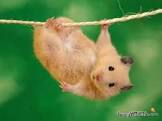
\includegraphics{./Figures/funny_mouse.jpg}
\caption{Hello world !}
\end{figure}

\chapter{Version control}\label{version-control}

This chapter is dedicated to version contol

\chapter{R package development}\label{r-package-development}

\section{Continuous integration}\label{continuous-integration}

\section{Unit testing}\label{unit-testing}

\section{Documentation}\label{documentation}

\bibliography{book.bib,packages.bib}


\end{document}
